\documentclass[11pt,article]{memoir}
\setsecnumdepth{none} % Turn off section numbering
\setcounter{tocdepth}{2}
\usepackage[utf8]{inputenc}
\usepackage[T1]{fontenc}
\usepackage{microtype}
\usepackage[dvips]{graphicx}
\setkeys{Gin}{width=.75\textwidth}
\usepackage[usenames,dvipsnames,svgnames,table]{xcolor}
\usepackage{times}
\usepackage[american]{babel}
\usepackage{amsmath}
\usepackage{amssymb}

% https://tex.stackexchange.com/questions/32598/force-latex-image-to-appear-in-the-section-in-which-its-declared
\usepackage[section]{placeins}

\usepackage[autostyle]{csquotes}

\usepackage[
breaklinks=true,colorlinks=true,
linkcolor=MidnightBlue,urlcolor=MidnightBlue,citecolor=MidnightBlue,% PDF VIEW
% linkcolor=black,urlcolor=black,citecolor=black,% PRINT
bookmarks=true,bookmarksopenlevel=2]{hyperref}

\usepackage{geometry}
\geometry{left=1in,right=1in,top=1in,bottom=1in}

% \usepackage{color}
\newcommand{\TODO}[1]{\textcolor{magenta}{\textbf{TODO: #1}}}

\usepackage[style=numeric,url=false]{biblatex}
\addbibresource{general_exam.bib}

% https://tex.stackexchange.com/questions/296476/cant-define-apa-as-bibstyle-undefined-control-sequence-argument-mkbibdatea
% \DeclareLanguageMapping{american}{american-apa}

\OnehalfSpacing

\begin{document}

{ % Title page
\sffamily
\centering
\Large

~\vspace{1in}

{\Huge
General Exam
}

\vspace{1in}

{\huge
Jason Portenoy
}

\vspace{.5in}

The Information School, University of Washington

\vspace{.5in}

May 2017

\vspace{1.5in}
{\small
Supervisory Committee: \\
Jevin D. West (chair) \\
Emma S. Spiro \\
Bill Howe \\
Benjamin Mako Hill (GSR) \\
}

\vspace{\fill}

} % end title page

\clearpage

\tableofcontents

\clearpage

% BEGIN INPUTS
% \emph{Please answer questions 1-4 in approximately 4-5 pages, not
including references. For question 5, provide a link to your
github/bitbucket repository with a 1-2 pg summary of what you did.}

\begin{enumerate}
\def\labelenumi{\arabic{enumi}.}
\item
  \textbf{What is community detection?} What are the common algorithms
  and history? How is this problem approached in various disciplines
  such as computer science, physics and network science? How does one
  evaluate a community detection algorithm? What are the top performing
  algorithms? Please give special attention to the evaluation part of
  this question.
\item
  \textbf{Applying community detection.} How is community detection
  being used in the wild? What kinds of questions does it try to answer?
  How is it being used in different disciplines, industry, etc?
\item
  \textbf{Visualizing communities.} What is the state of art for
  visualizing networks and specifically communities extracted from these
  networks? What are papers and labs developing these techniques? What
  are open challenges for visualizing network communities?
\item
  \textbf{Measuring our confidence in communities.} How does one measure
  confidence for a given cluster? How much would the partitions change
  with a different seed for a given algorithm or removal of a link or
  node in the raw network? To narrow your answer, please focus most of
  your answer on InfoMap since this is the algorithm you are most
  familiar with.
\item
  \textbf{Coding community detection algorithms.} To test your coding
  skills and your knowledge of community detection, recode in python a
  rudimentary version for minimizing the MapEquation, with a particular
  focus on the search algorithm. There are open source versions
  available (e.g., InfoMap) and you can refer to these, but I want you
  to focus on some of your own search solutions for minimizing the map
  equation. For example, you could employ a greedy algorithm or Monte
  Carlo based version. You can run this on a small example network. I do
  not expect a full scale code base. I just want to see some of your
  ideas for how you would minimize the MapEquation.
\end{enumerate}

% \clearpage
\section{History of community
detection}\label{history-of-community-detection}

Across many disciplines of science, it is common to encounter data that
can best be represented as a network, with entities linked to each other
in some meaningful way, such as through association or flow. These
entities are represented by \emph{nodes} or \emph{vertices} connected to
each other with \emph{links} or \emph{edges}. This overall
representation is known as a \emph{network} or \emph{graph}.\footnote{The
  term \emph{graph} generally refers to a mathematical representation of
  data, while \emph{network} usually has additional connotations related
  to the meaning and context associated with the data
  \autocite{porter_communities_2009}; however, as is the case with many
  terms in this area, the distinction is not always made and the two are
  often used interchangeably.} The idea of community detection as a
research topic comes from a basic intuition that there exist in these
networks groups of nodes that are structurally more related to each
other than they are to members of other groups.

The field of \emph{network science} has emerged recently to study this
and related topics. This field is highly interdisciplinary, comprising
physicists, applied mathematicians, computer scientists, sociologists,
and others. This interdisciplinarity arises both from the variety of
methods that can be applied, and the breadth of potential applications,
often requiring domain-specific knowledge
\autocite{porter_communities_2009}. Within this new field, the concept
of \emph{community} has been somewhat more formalized from the idea
above as a group of nodes (a \emph{subgraph}) with a high concentration
of edges connecting vertices within the group, and a low concentration
of edges with nodes outside the group
\autocite{fortunato_community_2010}.

The earliest analyses of communities were made by social scientists in
the early- to mid-twentieth century---for example Weiss and Jacobson's
analysis of the organizational structure of a government agency
\autocite{weiss_method_1955}. More developments were made by computer
scientists, who began developing graph partitioning algorithms in the
early 1970s to apply to problems in parallel computing and circuit
layout. In 2002, a seminal paper by Girvan and Newman
\autocite{girvan_community_2002} marked the entrance of the physics
community, and ushered in the modern age of community detection
\autocite{lancichinetti_community_2009}. The Girvan and Newman algorithm
introduced in their paper involved successively calculating the
\emph{edge betweenness}---the number of shortest path between all nodes
that run along the edge---of all edges, then removing the edge with the
highest betweenness and repeating. The idea is that the edges with the
highest betweenness centralities are the ones that connect communities,
and the communities can be separated by this divisive algorithm. This
work inspired the development of modularity as a quality measure (see
section on \protect\hyperlink{the-clustering-perspective}{the clustering
perspective} below). Since then, the field has seen rapid growth and the
development of many new methods.

\section{Community detection methods}\label{community-detection-methods}

What follows is an overview of some of the many community detection
methods currently in use. The overview follows the taxonomy laid out in
a recent paper by Schaub et al. \autocite{schaub_many_2017}. The authors
identify four different perspectives on the problem of community
detection: (i) \protect\hyperlink{the-cut-based-perspective}{the
\emph{cut-based perspective}}, (ii)
\protect\hyperlink{the-clustering-perspective}{the \emph{(data)
clustering perspective}}, (iii)
\protect\hyperlink{the-stochastic-equivalence-perspective}{the
\emph{stochastic equivalence perspective}}, and (iv)
\protect\hyperlink{the-dynamical-perspective}{the \emph{dynamical
perspective}}. The different perspectives represent different approaches
to the problem, often with different kinds of data, different methods,
and different goals. They also represent to some degree the different
research communities that have been working on the problem.

\TODO{Add a note about how this might not be the only way to classify the problem space, but it is one way. It does not divide the methods cleanly, but neither do other classification. This is maybe because there are so many connections between methods. Link to discussion in the evaluation section on the need for splitting the problem up.}

\hypertarget{the-cut-based-perspective}{\subsection{The cut-based
perspective}\label{the-cut-based-perspective}}

Some of the earliest work in community detection was in the area of
circuit layout and design. A circuit can be represented as a graph
describing the signal flows between its components. The efficient layout
of of a circuit depends on partitioning the circuit into a fixed number
of similarly sized groups with a small number of edges between
groups---these inter-group edges are known as the \emph{cut}. Similar
problems can be found in load scheduling and parallel computing, where
tasks must be divided into different portions with minimal dependencies
between them. These need for these methods led to the development of the
Kernighan-Lin algorithm in 1970 \autocite{kernighan_efficient_1970},
which has become a classical method that is still frequently used. It
starts with an initial partition and attempts to optimize a quality
function \(Q\) representing the difference between intra-cluster edges
and inter-cluster edges, by swapping equal-sized subsets of vertices
between groups. The method works best if it starts with a decent initial
partition, so in modern use it is often used to refine partitions
obtained using other methods \autocite{fortunato_community_2010}.

The cut-based perspective has also seen the development of spectral
methods for graph partitioning. The spectrum (eigenvalues) of a graph's
adjacency matrix tend to be related to the connectivity of the graph,
and the associated eigenvectors can be used for both cut-based
partitioning and clustering. These methods typically make use of the
Laplacian matrix \(L\) of a connected graph \(G\): \(L = D - A\) where
\(A\) is the adjacency matrix of \(G\) and \(D\) is the diagonal degree
matrix with \(D_{ii} = \sum_{j}{A_{ij}}\). The \emph{Fiedler vector} is
the second-smallest eigenvector associated with the Laplacian matrix
\(L\); the spectral bisection method uses this vector to quickly
partition a graph into two groups with a low cut size
\autocite{fiedler_algebraic_1973}.

A cut-based measure for the quality of a partition is the
\emph{conductance}. The conductance of a subgraph \(S \in V\) for a
graph \(G(V, E)\) is:
\[\phi(S) = \frac{c(S, V \setminus S)}{\min(k_S, k_{V \setminus S})}\]
Where \(c(S, V \setminus S)\) is the cut size of \(S\), and \(k_S\) and
\(k_{V \setminus S}\) are the total degrees of \(S\) and the rest of the
graph, respectively \autocite{schaeffer_graph_2007}. While this measure
was originally used globally to optimize a bisection of a graph, it has
also seen use as a local quality function to find good clusters around
certain nodes; in this way it can also be viewed as part of the
clustering perspective \autocite{schaub_many_2017}. Conductance has its
roots in computer science, and its use in network science appears still
to be especially popular in the computer science community
\autocites{schaeffer_graph_2007}{yang_defining_2015}.

\hypertarget{the-clustering-perspective}{\subsection{The clustering
perspective}\label{the-clustering-perspective}}

The clustering perspective comes from the world of data clustering, in
which data points are thought of as having ``distance'' between each
other based on their (dis)similarity, and the goal is to group together
data point that are close to each other. For community detection, this
distance is in relation to the connections between nodes in the network.
This perspective is related to but different from the cut-based
perspective above, which seeks to place divisions among the nodes so as
to form balanced groups with weak connections between groups.

A classical method with this perspective is \emph{hierarchical
clustering}, which when used on graphs yields a hierarchical
partitioning that can be viewed as a dendrogram. The common method uses
an agglomerative approach in which each node starts in its own cluster,
and they are joined together one by one based on some similarity measure
calculated using the graph's adjacency matrix. This approach to
community detection has several weaknesses. It necessarily infers a
hierarchical community structure even if one does not exist; the
hierarchy is not always easy to interpret; it often misclassifies nodes,
especially nodes with only one neighbor, which it tends to put it in its
own cluster; and it does not scale well to large networks
\autocite{fortunato_community_2010}.

\TODO{modularity}

\hypertarget{the-stochastic-equivalence-perspective}{\subsection{The
stochastic equivalence
perspective}\label{the-stochastic-equivalence-perspective}}

\hypertarget{the-dynamical-perspective}{\subsection{The dynamical
perspective}\label{the-dynamical-perspective}}

\subsection{Future/open problems}\label{futureopen-problems}

\TODO{hierarchical. overlapping.}

\clearpage
\hypertarget{evaluation}{\section{Evaluation of community detection
methods}\label{evaluation}}

\protect\hyperlink{evaluation}{}

The lack of consensus on exactly what a community is and what is meant
to be achieved by its detection has presented problems for the
evaluation of community detection methods. Still, attempts have been
made to systematically evaluate the performance and output of different
methods.

Evaluating the results of any community detection method can be thought
in terms of either \emph{internal} or \emph{external} validity. Measures
of \emph{internal} validity evaluate the output of a clustering
algorithm according to some quality measure that uses only the
properties of this output; these include modularity
\autocite{newman_finding_2004}, minimum description length
\autocite{rosvall_map_2010}, and conductance
\autocite{leskovec_empirical_2010}. These measures are designed to
measure how well the communities identified by a method adhere to some
mathematical definition of what a proper community structure should look
like. The problem with using these measures to evaluate and compare
methods is that these measures often serve as the objective functions
for the very algorithms we want to evaluate. While it may be useful to
use these quality measures to compare algorithms that are trying to
optimize the same function, it may not be fair to compare more broadly
than this. As there is no strict mathematical definition for a
community, different algorithms use different quality functions to
surface community structure, and those algorithms that optimize for
whatever measure we are using to evaluate would have an unfair
advantage. Some of these quality measures are discussed in the previous
section on existing community detection algorithms.

Because of this, much of the work around evaluating community detection
methods has focused on \emph{external} validity measures, in which the
input is a network with a known community structure. The evaluation in
this case measures how well the community detection method matches this
ground truth. These ``gold standard'' networks used for evaluation are
either (1) synthetic benchmark networks created with planted
communities, or (2) real-world networks with known metadata which are
treated as ground-truth communities. In either case, the results of a
community detection algorithm can be evaluated against the expected
structure using some comparison measure.

\hypertarget{comparison-measures}{\subsection{Comparison
measures}\label{comparison-measures}}

Evaluating a community detection method against either a synthetic
benchmark network or a real-world network with known community structure
requires some measure of comparison between the clustering found by the
method and the ground truth clustering. The popular measures that have
been adopted fall into one of three categories: (1) measures based on
\emph{pair counting}, (2) measures based on \emph{set matching}, or (3)
measures based on \emph{information theory}
\autocites{meila_comparing_2007}{vinh_information_2010}. These are all
general measures comparing data (not just network) clusterings; they
work by viewing the network as data points with communities as cluster
assignments.

\emph{Pair counting measures} work by taking every possible pair of
nodes in the network and classifying them based on their co-occurrence
in the clusterings. Each of these categories is then counted:

\begin{itemize}
\tightlist
\item
  \(N_{11}\): the number of pairs that co-occur in the same cluster in
  both clusterings
\item
  \(N_{00}\): the number of pairs that do not co-occur in either
  clustering
\item
  \(N_{10}\) or \(N_{01}\): the number of pairs that co-occur in one
  clustering but not the other.
\end{itemize}

Examples of measures that use these counts include the Fowlkes-Mallows
index \autocite{fowlkes_method_1983} and the Rand index
\autocite{rand_objective_1971}. The Rand index, for example, is the
ratio of pairs correctly classified in both clusterings to the total
number of pairs:

\[\frac{N_{11} + N_{00}}{N_{11} + N_{00} + N_{10} + N_{01}}\]

This measure has a value between zero and one, with one representing
perfect agreement between the clusterings and zero representing no
agreement whatsoever. In practice, it is rare to see values on the lower
end of this range, so a transformation is usually applied that sets a
baseline that accounts for chance---this is known as the adjusted Rand
index.

\emph{Set matching measures} compare clusterings by finding matches
between the clusters---for example, by treating the cluster assignments
as labels and calculating the classification error rate. This approach
has problems when the two clusterings to be compared have different
numbers of clusters, however. Even within the clusters that match, these
measures only consider the matched part of each cluster pair, leaving
out the parts that do not match. For these reasons, these measures are
not very widely used
\autocites{meila_comparing_2007}{vinh_information_2010}.

\emph{Information theoretic measures} use elements of information theory
to compare clusterings. The \emph{entropy} \(H(\mathcal{C})\) of
clustering \(\mathcal{C}\) is the average amount of information (in
bits) needed to encode and transmit each label. The \emph{mutual
information} between two clusterings \(\mathcal{C}\) and
\(\mathcal{C'}\) is the entropy of \(\mathcal{C}\) minus the conditional
entropy of \(\mathcal{C}\) given \(\mathcal{C'}\), or vice versa:
\(H(\mathcal{C}) - H(\mathcal{C}|\mathcal{C'}) = I(\mathcal{C}, \mathcal{C'}) = H(\mathcal{C'}) - H(\mathcal{C'}|\mathcal{C})\).
If we let \(P(k), k = 1, \ldots, K\) and \(P'(k'), k' = 1, \ldots, K'\)
be the random variables associated with the clusterings \(\mathcal{C}\)
and \(\mathcal{C'}\), respectively, and \(P(k, k')\) be the joint
probability---the probability that a point belongs to \(C_k\) in
clustering \(\mathcal{C}\) and to \(C'_{k'}\) in clustering
\(\mathcal{C'}\), then:

\[I(\mathcal{C}, \mathcal{C'}) = \sum_{k=1}^{K} \sum_{k'=1}^{K'} P(k, k') \log \frac{P(k, k')}{P(k) P'(k')}\]

The mutual information tells us, on average, how much knowing the
cluster assignment of a point in \(\mathcal{C}\) reduces our uncertainty
of which cluster it belongs to in \(\mathcal{C'}\). Several variations
of the mutual information measure have been proposed, including
normalized versions that are meant to vary between 0 (the clusterings
are independent of one another) and 1 (the clusterings are identical);
and versions adjusted for chance \autocite{vinh_information_2010}.
Another measure is the \emph{variation of information}:

\[
\begin{aligned}
VI(\mathcal{C}, \mathcal{C'}) &= H(\mathcal{C}) + H(\mathcal{C'}) - 2I(\mathcal{C}, \mathcal{C'}) \\
                                                            &= H(\mathcal{C}|\mathcal{C'}) + H(\mathcal{C'}|\mathcal{C})
\end{aligned}
\]

Finally, Lancichinetti et al. proposed a version of the normalized
mutual information that can handle the case of \emph{covers},
clusterings in which a node can be assigned to more than one cluster
\autocite{lancichinetti_detecting_2009}. While the authors point out
that their measure is not a true extension of normalized mutual
information because it gives different values when used to compare
normal ``hard'' clusterings, they contend that the difference is small
\autocite{lancichinetti_community_2009}.

\hypertarget{synthetic-benchmark-networks}{\subsection{Synthetic
benchmark networks}\label{synthetic-benchmark-networks}}

Evaluating community detection methods can mean comparing their results
with the expected results on some network with known community
structure, using the above similarity measures. One way to get such a
network is by using computer-generated synthetic benchmarks networks,
which are created with some notion of built-in community structure.
While there is no clear consensus on exactly what this structure should
look like, some standard benchmarks have emerged.

The \emph{planted \(\ell\)-partition model} is one method of generating
such a benchmark network. In this model, a graph is created with a
certain number (\(\ell\)) of clusters, each having the same number of
nodes. Nodes are connected with edges to other nodes in the same cluster
with probability \(p_{in}\), and to nodes in other clusters with
probability \(p_{out}\); as long as \(p_{in} > p_{out}\), the graph has
some community structure. The version of this model that has become
standard is known as the Girvan and Newman (GM) benchmark
\autocite{girvan_community_2002}. In this version, the number of
clusters is set at 4, with 32 nodes per cluster, and an average total
degree of 12. The parameter one uses to change how pronounced is the
community structure of the generated network is \(z{out}\)---the
expected external degree of a node. (Because the expected total degree
of a node is fixed, \(z_{in}\)---the expected internal degree of a
node---depends on \(z_{out}\)). As \(z_{out}\) increases, the community
structure of the graph becomes less apparent, until
\(z_{out} = z_{in} = 8\), in which case the internal and external
degrees are equal (see Fig.~\ref{fig:gn_benchmarks}). Many algorithms
are able to properly identify communities up to this limit
\autocite{fortunato_community_2010}.

\begin{figure}
\centering
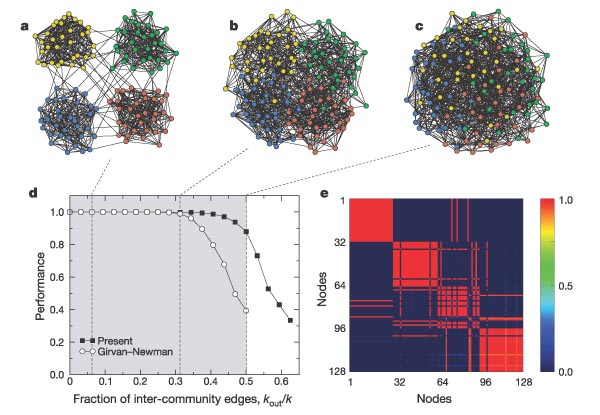
\includegraphics{img/guimera2005_fig1_gm-benchmarks.jpeg}
\caption{Examples of the Girvan-Newman benchmark. From left to right,
the parameter \(z_{out}\) increases (and \(z_{in}\) decreases), and the
community structure becomes less apparent. In (a) \(z_{in}=15\); in (b)
\(z_{in}=11\); and in (c) \(z_{in} = z_{out} = 8\) and the four clusters
are not visually apparent. Image from
\autocite{guimera_functional_2005}.}\label{fig:gn_benchmarks}
\end{figure}

The weakness of the GN benchmarks and the planted \(\ell\)-partition
model in general lies in assumptions that all communities have the same
size and all nodes have the same degree on average. Real-world networks
tend to exhibit skewed, power-law-like distributions for cluster size
and node degree. Lancichinetti et al. have taken steps to address these
issues with their LFR benchmark, which is generally seen as an
improvement over the GN benchmark
\autocites{lancichinetti_benchmark_2008}{fortunato_community_2010}. When
an LFR network is generated, both the degree and cluster size are
assumed to have power law distributions, with exponents \(\gamma\) and
\(\beta\), respectively. The mixing parameter \(\mu\) specifies, for
each node, the fraction of its links that go outside its community. A
graph of \(N\) vertices is generated using a configuration model which
assigns links given the proper degree sequence; the graph is then
rewired with an iterative algorithm until it can be assigned a community
structure with the proper parameters.

\subsection{Evaluation on real-world
networks}\label{evaluation-on-real-world-networks}

A second approach to evaluate community detection methods is to use some
real-world network data and compare the results of the method against
known metadata attributes, which are treated as ground-truth community
structure. The most famous of these networks is the Zachary karate club
dataset \autocite{zachary_information_1977}, which is a network
representation of the social interactions between 34 members of a
university karate club. A conflict between the club president and the
instructor resulted in the formation of two groups of members who had
allegiance to one leader or the other. Community detection methods can
be judged according to how well they are able to infer this group
division from the network structure alone. This network has become so
widely used as a benchmark in network science that researchers who are
first to use it as an example at a conference are awarded a trophy and
inducted into the prestigious ``Zachary Karate Club Club.''\footnote{See
  \url{http://networkkarate.tumblr.com/}} Several other networks have
also emerged as standard benchmarks: Lusseau's network of interaction
between 62 bottlenose dolphins in New Zealand's Doubtful Sound is
compared against a biological classification
\autocite{lusseau_emergent_2003}; and a network in which nodes represent
college football teams and edges represent games played between them is
compared against the known conference divisions of the teams
\autocite{girvan_community_2002}.

The assumption that known metadata can be equated with community
structure has recently begun to be called into question, amid several
findings that most community detection algorithms tend to do a fairly
poor job of recovering these classifications on many large networks
\autocites{yang_defining_2015}{hric_community_2014}. This may represent
something of a crisis for the field.

A very recent paper by Peel et al. breaks down these issues
\autocite{peel_ground_2017}, providing a very interesting and
provocative perspective. While it has been assumed that a method's
failure to recover the metadata associated with the network means that
the method has performed poorly, the authors point out that there are
actually three alternative interpretations: (i) that the metadata do not
actually correspond with network structure, (ii) that the metadata
correspond to a different aspect of the network structure than that
revealed by the community detection method, or (iii) that the network
actually has no detectable community structure. The authors propose a No
Free Lunch theorem for community detection, claiming that no one method
can outperform any other on all cases, implying that methods that have
an advantage for a certain set of cases will have decreased performance
in other cases. They stress that this does not imply that community
detection is a useless endeavor, but they do contend that it is
impossible to find one optimal method, and that efforts should instead
be put into understanding the problem space of different community
detection tasks, so that different algorithms can be developed for each
one. The recent review paper by Schaub et al.
\autocite{schaub_many_2017} is one example of this kind of effort,
classifying and distinguishing the different perspectives on community
detection.

The authors of this study introduce two interesting new statistical
methods to address cases (i) and (ii) in the paragraph above. The first
identifies the extent to which the metadata relates to the network
structure by comparing the entropies of two probabilistic models: one
representing the metadata partitions, and the other a null model with
random permutations of the metadata (this null model preserves network
structure and relative frequencies of metadata values but removes the
correlation between the two). The second statistical method is meant to
shed light on the relatedness between the structural aspects of the
metadata versus the structural aspects that a community detection
algorithm identifies. It does this by imposing a constraint on the
community detection algorithm that fixes some portion of the community
structure produced based on the metadata partitions. By varying this
constraint, one can explore (visually, using a graph) how the imposition
of the metadata affects the likelihood of the community detection
method. Both of these methods are general enough to work with any sort
of probabilistic generative network model; the authors implement them
using stochastic blockmodels (see previous section on community
detection methods), calling the first method the blockmodel entropy
significance test (BESTest), and the second one the neoSBM.

\TODO{2002 girvan and newman paper recognized the idea that metadata might not always be related to network structure. see my note in zotero}

\TODO{Maybe think some more about implications of how community detection is an ill posed problem, and the No Free Lunch theorem}

\subsection{Results of comparative analyses of
algorithms}\label{results-of-comparative-analyses-of-algorithms}

A 2009 paper by Lancichinetti and Fortunato
\autocite{lancichinetti_community_2009} has gained some acceptance in
the network science community as a comparative analysis of the
performance of some of the most popular community detection algorithm.
The 12 algorithms studied included most of those previously discussed
(see section ``\protect\hyperlink{community-detection-methods}{Community
detection methods}''), including the original Girvan-Newman algorithm,
several greedy and more exhaustive modularity-optimizing algorithms, an
Expectation-Maximization Bayesian model-fitting approach similar to
stochastic block models, a spectral algorithm, the Markov cluster
algorithm popular in bioinformatics, and the flow-compression-based
Infomap algorithm of Rosvall and Bergstrom, among several others. They
also included one algorithm that can find overlapping partitions, called
Cfinder.

The algorithms were tested on random graphs generated using the LFR
method (see section
``\protect\hyperlink{synthetic-benchmark-networks}{Synthetic benchmark
networks}''; these benchmark graphs are more rigorous than the
Girvan-Newman benchmarks that came before. The results were compared
using their variant of normalized mutual information (see section
``\protect\hyperlink{comparison-measures}{Comparison measures}'').
Briefly, the results were as follows: The original Girvan-Newman
algorithm suffered from too many performance issues to be considered,
failing to finish on most networks (the authors included this method
mostly for historical reasons; the other methods are more modern and
improved). The modularity-based methods tended to suffer from that
approaches resolution limit (see section
``\protect\hyperlink{the-clustering-perspective}{The clustering
perspective}''), failing to detect smaller planted communities on larger
graphs. The authors concluded that Infomap was overall the best
performing algorithm, with good performance on different sized graphs,
and also directed and weighted graphs. It was also one of the fastest
methods, along with the Louvain method---the authors were able to test
these two on larger graphs (up to 100,000 nodes), and only Infomap
maintained good performance. The study did not study hierarchical
partitions, or the overlapping or higher-order versions of Infomap.

The authors also test the methods on random graphs. An algorithm taking
as input a random graph, in which every pair of nodes having an equal
probability of being linked, should not find a community structure, but
this is not always the case (see section
\protect\hyperlink{confidence-in-communities}{``Confidence in
communities''}). Methods based on modularity fall short here, finding
some communities in random graphs. Infomap tends to perform better,
finding a single module comprising all nodes. However, Infomap still
does find some community structure when the average degree of the nodes
is low---i.e., the graph is sparse. This could pose a problem, as many
real-world graphs are sparse.

A recent paper by Emmons et al. \autocite{emmons_analysis_2016} is an
update to the Lancichinetti and Fortunato paper. Computation has
advanced, and they were able to test LFR benchmark graphs up to 1
million nodes on four algorithms: Louvain, Smart Local Moving (SLM),
Infomap, and Label Propagation. Louvain and SLM are both
modularity-optimizing methods that work on large networks; Label
Propagation is a method equivalent to the Pott's model approach (another
clustering method I have not extensively investigated in this work). The
authors found results that contradict Lancichinetti and Fortunato, with
Louvain (and SLM) outperforming Infomap. The most likely reason for this
is discussed in the results: the authors choose to use benchmark graphs
with relatively large clusters, so the resolution limit of the
modularity-based methods (Louvain and SLM) actually work in their favor,
when usually they are a detriment. The results of Infomap are based on
the lowest level of the hierarchical partitioning---at this level
Infomap finds smaller clusters than those planted, leading to the lower
information recovery scores.

\TODO{remark on how LFR benchmarks are based on SBMs, so they would be expected to score best. can find this in fortunato and hric 2016 (and also i think in schaub 2017)}

\subsection{Visualization}\label{visualization}

\clearpage
\section{Applications of community
detection}\label{applications-of-community-detection}

The extensive work behind developing and validating methods for
community detection is presumably meant to work toward a goal of using
community detection for some concrete applications. In this area, the
field shows its (young) age---it is somewhat difficult to find published
examples where the methods have been applied to solve a specific problem
or gain significant new insight into a system. Below, I discuss some of
the examples that do exist in the research literature, in the fields of
\protect\hyperlink{social-network-analysis}{social network analysis},
\protect\hyperlink{networks-of-scholarship}{networks of scholarship},
\protect\hyperlink{biological-networks}{biological networks}, and
\protect\hyperlink{other-research}{others}. Besides published research,
I speculate on the (mostly unpublished) applications of community
detection outside of academia, and present an example of using community
detection in the context of a small data science project to address a
question of interest.

\hypertarget{social-network-analysis}{\subsection{Social network
analysis}\label{social-network-analysis}}

Social networks often contain intuitive and potentially interesting
community organization, so it is not surprising that there has been
interest in applying community detection to various forms of social
data. The enormous popularity of online social network platforms like
Facebook and Twitter have made detailed social network data available at
a massive scale. These data are not available equally to
everybody---most popular social networking applications are proprietary
and much of their data are reserved for internal research. It is likely
that these companies are using community detection to explore patterns
in their data, but not publishing all of their results.

One published study of Facebook was conducted by Traud et al.
\autocite{traud_social_2012}. They examined the Facebook friend network
from 100 American colleges and universities (at the time of this study,
Facebook was restricted to these institutions). They performed community
detection using several modularity-optimizing techniques and compared
the community structure against several (self-reported) categorical
demographic variables---gender, class year, high school, major, and
residence. Fig.~\ref{fig:facebook} shows a visualization of community
structure with class year---the variable most strongly associated with
community structure. The authors find some patterns that we might
reasonably expect, such as class year being associated with friend
communities, and high school being more associated with communities at
larger institutions (where one is more likely to find multiple people
from the same high school). They also identify some patterns that would
be interesting to study further, such as that females were more likely
to have friends within their same residence.

\begin{figure}
\centering
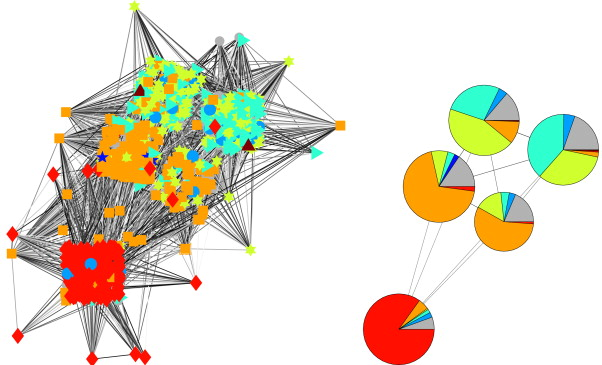
\includegraphics{img/traud2012_fig2_facebook.jpg}
\caption{Community structure from the Reed College Facebook friend
network. On the left, colors and shapes of nodes indicate different
class years. On the right, the communities are condensed into pies. The
size of the pies correspond to the number of nodes, and darker edges
mean more connections between communities. A correlation between class
year and community structure can be seen. Figure from
\autocite{traud_social_2012}.}\label{fig:facebook}
\end{figure}

\begin{figure}
\centering
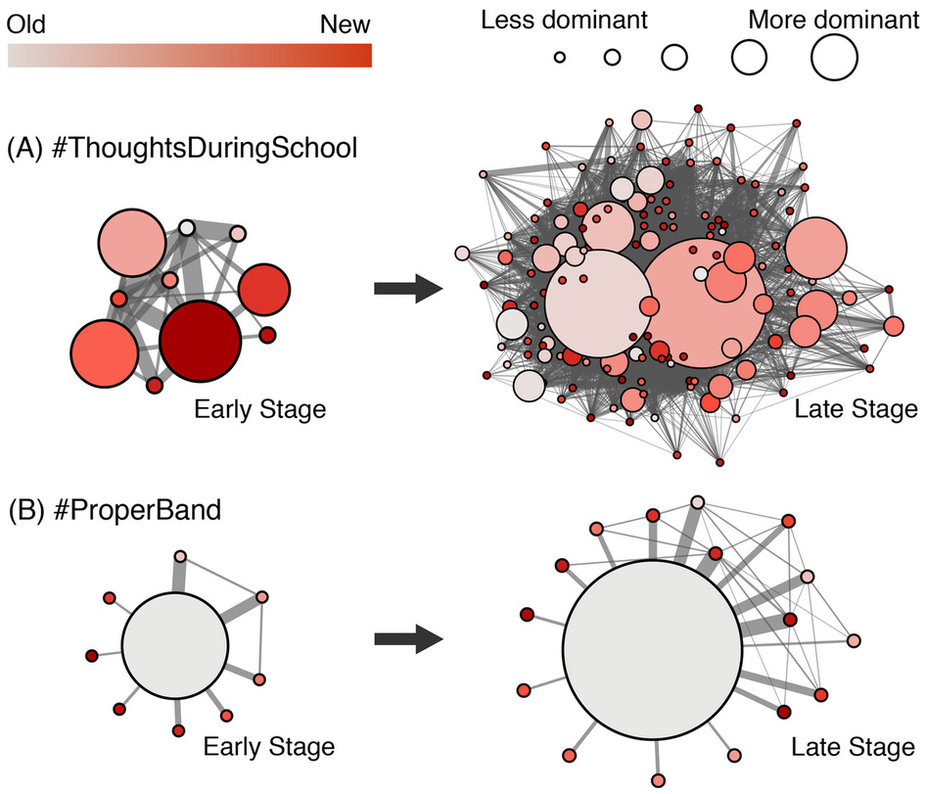
\includegraphics{img/weng2013_fig4_viraltwitter.jpg}
\caption{The evolution of a viral meme (A) vs.~a non-viral meme (B).
Each node is a community, with size proportional to the number of tweets
produced by the community, and color indicating the relative time that
the hashtag was first used by the community. Figure from
\autocite{weng_virality_2013}.}\label{fig:viraltwitter}
\end{figure}

Weng et al. \autocite{weng_virality_2013} used community detection to
study the virality of memes on Twitter. Since the question of interest
was one of information flow, they used Infomap, a flow-based community
detection method (see subsection
``\protect\hyperlink{the-dynamical-perspective}{The dynamical
perspective}'' in section
``\protect\hyperlink{community-detection-methods}{Community detection
methods}'' above). They identified communities in networks of
reciprocal-follower relationships among Twitter users.
Fig.~\ref{fig:viraltwitter} shows the evolution of a viral meme vs.~a
non-viral meme (here a meme corresponds to a hashtag), with the
communities represented as nodes. The results suggest that a meme that
is less concentrated in one community is more likely to spread, and that
community structure might be helpful in predicting the virality of
memes. They go on to apply a random forest classifier for new memes that
takes into account community features, and find that these features are
helpful in predicting whether a meme will go viral.

\hypertarget{networks-of-scholarship}{\subsection{Networks of
scholarship}\label{networks-of-scholarship}}

The collective human endeavor of knowledge generation and organization
can be represented as a directed network of scholarly publications with
citations between them. The citation links between publications can been
viewed as a proxy for influence or information flow. De Solla Price
recognized the potential of this representation in the mid 20th century
\autocite{de_solla_price_networks_1965}, and over the years much work
has been done in this meta-scientific research area, which has been
given terms such as ``bibliometrics,'' ``scientometrics,'' and ``science
of science''.
\TODO{Communities represent fields of study. Dynamic methods are good for this. They analyzed JSTOR. Can identify related literature and possibly unknown connections. Recommendation paper. Cultural holes? Mapping change--neuroscience? image of flows between disciplines? image of neuroscience alluvial?}

\hypertarget{biological-networks}{\subsection{Biological
networks}\label{biological-networks}}

Many biological systems can be thought of as structured interactions
between functional elements, often with (possibly hierarchical) modular
structure. It is natural to think of these systems as networks, and to
see promise in the prospect of identifying communities in this network
representation.

Protein-protein interaction networks are constructed from data collected
in experiments that identify molecular interactions between proteins.
Community detection on these networks, for example using the
Girvan-Newman edge betweenness method, has been shown to be effective in
identifying what are known as ``functional modules'' in these
networks---groups of proteins that interact in the service of a
particular cellular process. Clusters found in these networks correspond
to existing annotations, suggesting promise for the automated analysis
of experiments. These methods were also found to be robust against false
positive interactions, which is important considering that experimental
results can contain considerable noise \autocite{dunn_use_2005}. Chen
and Yuan \autocite{chen_detecting_2006} integrated multiple protein
interaction datasets containing hundreds of microarray expression
profiles for \emph{Saccharomyces cerevisiae} (brewer's yeast) to form a
weighted graph, in which the weights correspond to dissimilarity between
genes' expression profiles. By classifying the genes into functional
modules using a modified version of the Girvan-Newman method, they were
able to predict the function of the as-yet not annotated yeast gene
\emph{YLR419w} to be chromosome segregation.

Another biological network that has been studied is the directed network
of neuronal connections---the ``connectome''. Dynamically-minded
community detection methods (see subsection
``\protect\hyperlink{the-dynamical-perspective}{The dynamical
perspective}'' in section
``\protect\hyperlink{community-detection-methods}{Community detection
methods}'' above) are especially relevant for these networks as the
connectome represents a system of information flow, which is what these
methods model. Bacik et al. \autocite{bacik_flow-based_2016} grouped the
neurons of \emph{C. elegans} using flow-based methods. These detected
communities showed good agreement with previous understanding of
functional neuronal groups. They were then able to perform \emph{in
silico} ablations of neurons---computer simulations in which they
removed nodes and looked at the resulting disruption on community
structure. By doing this, they identified neurons important to the
network flow, and presumably important to the neuronal function of the
organism. These included neurons known to be important, as well as
previously uninvestigated neurons that can be candidates for future
study.

\TODO{Metabolic networks? Maybe can skip this.}

\hypertarget{other-research}{\subsection{Other examples in the research
literature}\label{other-research}}

\TODO{Legislative networks: see porter paper}

\begin{itemize}
\tightlist
\item
  \autocite{lupu_trading_2013}: States that trade with each other are
  known to have less conflict with each other. This paper extends this
  to trade communities, so that states that don't trade with each other
  that much, but are indirectly linked by trade, also have less conflict
  with each other. They use community detection (via modularity
  maximization) to test this theory.
\end{itemize}

\TODO{see fortunato paper. see porter paper.}

\subsection{Non-research applications}\label{non-research-applications}

\TODO{terrorism? crime? marketing? maybe not reflected in the research. Community detection to identify fraud events in telecommunication networks.}

\clearpage
\hypertarget{visualization}{\section{Visualizing community structure in
networks}\label{visualization}}

\protect\hyperlink{visualization}{}

A recent paper in the EuroVis conference by Vehlow et al.
\autocite{vehlow_state_2015} gives a thorough overview of the state of
the art in visualizing group structure in networks. In addition to
giving a literature survey as well as a taxonomy for these
visualizations, they provide a detailed curated bibliography at
\url{http://groups-in-graphs.corinna-vehlow.com/}. There one finds a
visualization tool for exploring the surveyed literature on this topic,
and also the full tagged bibliography available for download as a BibTeX
file.

One question was somewhat difficult to answer given the format this
bibliography was presented: What are the labs doing work in this area?
While the bibliography presented important papers related to the topic,
they were not organized by lab. In order to address this question, I
perform a community analysis and visualization on the bibliography data
provided. The visualization is available \ldots{} I also use this
endeavor as a first-hand illustration of the utility and challenges
around detecting and visualizing communities in network data.

Starting with data on papers and seeking insight into the organization
of research in different labs seemed like an appropriate situation to
apply community detection methods. I first constructed a co-authorship
network in which nodes represent authors, and weighted links represent
the number of papers in which a pair appear as authors. In addition, I
used the Microsoft Academic API \TODO{cite} to attempt to assign an
affiliation to each author by querying Microsoft Academic Graph for the
author and retrieving the most prevalent affiliation for that author
among the papers returned. I then used
\protect\hyperlink{the-dynamical-perspective}{Infomap} to find a
hierarchical clustering of the nodes. To visualize the results, I
include only the connected components with at least 10 nodes. Each node
represents a single author; \TODO{NUMBER} authors appear in the
visualization. The sizes of the nodes correspond to the amount of
flow---the relative importance of an author in this co-authorship
network. The color of each node is assigned based on the top-level
cluster assignment of that author. Clicking on any node of a connected
component will shift the focus to that component, and reassign colors,
this time based on the bottom-level cluster assignment. I also provide a
search box which makes it easier to find specific authors or
affiliations.

I represent the co-authorship network as a node-link diagram, which is a
very common way of visualizing networks. The nodes are visualized using
a force-directed algorithm, in which forces of attraction and repulsion
are applied to nodes and links and then placed so as to minimize the
energy. Interestingly, the force-directed layout has been shown to be
equivalent to the commonly used modularity quality function for
communities \TODO{cite}---this is why a visualization of a network that
uses this layout can have show implicit community structure by grouping
similar nodes together visually.

Using this system can help to identify some of the key researchers in
this area and the relationships between them. To find the labs, I can
search the web for their lab or university websites. By doing this, I
was able to find a number of labs doing interesting work.

One community that pops out appears in the middle of the largest
connected component, with several large and well-connected nodes.
Perhaps unsurprisingly, this community represents the authors of the
survey paper (and the curators of the bibliography data behind the
visualization). This is the University of Stuttgart Visualisation
Research Centre (VISUS), and includes Daniel Weiskopf, Fabien Beck and
others. It also used to include former PhD student and lead author of
the survey paper Corinna Vehlow. An interesting recent paper from this
lab is \autocite{vehlow_visualizing_2015}, in which dynamically evolving
community structure is visualized as rectangular blocks (in a way
resembling the alluvial diagrams in Rosvall and Bergstrom
\autocite{rosvall_mapping_2010} see Fig.~\ref{fig:alluvial}), and these
are combined with node-link representations of the community subgraphs.

Close to the Stuttgart lab is the team at LaBRI at the University of
Bordeaux, France. Researchers here include Romain Bourqui and David
Auber. Dr.~Auber appears to work closely with researchers at the
University of British Columbia including Tamara Munzner and Daniel
Archambault. An interesting paper from the LaBRI group is
\autocite{sansen_adjasankey:_2015}, where one technique they use to show
hierarchical structure involves assigning similar color to similar
nested groups.

Other groups can be seen in the largest connected component. A group of
researchers appears as a maroon community; this is the MArVL group at
Monash University in Melbourne, Australia, which includes Kim Marriott
and Tim Dwyer (I have seen Tim's work before---he created cola.js, a
constraint-based graph visualization layout that works with D3). The UC
Davis Center for Visualization appears as a mostly blue community. The
University of Arizona Graph and Map Algorithm (GAMA) Lab, headed by
Stephen Kobourov, is well connected in the component. An interesting
paper out of this last lab is \autocite{gansner_gmap:_2010}, in which
communities are visualized to look like cartographic maps. This method
has a pleasing aesthetic that people might find preferable to the
standard node-link diagram, as many people are turned off by the
``hairball'' that tends to result from the standard approach. Indeed,
the authors use their mapping technique to visualize a co-authorship
network, and this may be a superior way to visualize this data than what
I have done. Another paper \autocite{saket_map-based_2015} found that
the cartographic map technique improved people's recall of data.

Some labs are represented in the smaller components as well. One such
component contains two labs in China---the Tong Ji Intelligent Big Data
Visualization Lab, headed by Nan Cao; and the VisLab at Hong Kong
University, headed by Huamin Qu. One paper from the VisLab is
\autocite{wu_interactive_2015}, in which contour overlays using Voronoi
cells are superimposed over nodes to show communities.

\TODO{note that there might be errors due to using names as unique IDs}

\TODO{Results of exploration. Talk about labs. Highlight some interesting work coming out of labs. }

\TODO{Brushing and linking. Cao et al. g-miner. abello et al. ask-graphview.}

\TODO{Contours. Wu et al (in hong kong univ VisLab) use voronoi overlays}

\TODO{Back to vis. Describe taxonomy}

\TODO{Briefly talk about tasks and evaluation}

\TODO{Discuss open problems}

\TODO{Interestingly, modularity and force-directed layout are the same -- Noack 2009}

\begin{itemize}
\tightlist
\item
  Labs:

  \begin{itemize}
  \tightlist
  \item
    Tong Ji Intelligent Big Data Visualization Lab
    (\url{https://idvxlab.github.io/}) headed by Nan Cao
  \item
    Hong Kong University's VisLab headed by Huamin Qu. Together with
    above (Tong Ji) in their own component
  \item
    MArVL: Monash Adaptive Visualisation Lab
    (\url{http://marvl.infotech.monash.edu/members/}) headed by Kim
    Marriott (includes Tim Dwyer)
  \item
    University of Stuttgart Visualisation Research Centre
    (\url{http://www.visus.uni-stuttgart.de/en/institute.html}) includes
    Prof Daniel Weiskopf, Research associate Dr.~Fabien Beck, and former
    PhD student Corinna Vehlow (these are the authors of the STAR paper)
  \item
    UC Davis Center for Visualization headed by Kwan-Liu Ma. there are
    problems with their website
  \item
    University of Arizona Graph and Map Algorithm (GAMA) Lab headed by
    Stephen Kobourov
  \item
    Johannes Kepler University Linz -- Institute of Computer Graphics --
    Deputy head of the institute Marc Streit. off on its own connected
    component.
  \item
    David Auber at LaBRI works a lot with Daniel Archambault and Tamara
    Munzner at UBC
  \end{itemize}
\end{itemize}

\TODO{Appendix describing methods?}

\clearpage
\hypertarget{confidence-in-communities}{\section{Confidence in
communities}\label{confidence-in-communities}}

\protect\hyperlink{confidence-in-communities}{}

\subsection{Statistical significance}\label{statistical-significance}

Although it is counterintuitive, completely random graphs, when viewed a
certain way, can be seen to have community structure. In a random graph,
known as an Erdős--Rényi graph \autocite{erdos_evolution_1960}, every
node has an equal probability of being linked to every other node.
Fig.~\ref{fig:randomcommunities} shows how a random graph can show group
structure. The top left shows the adjacency matrix of a random graph
with nodes in arbitrary order; this looks like random white noise. By
rearranging the order of the nodes in the same random graph, as in the
other panes of the figure, a community structure becomes apparent. This
is not actual community structure we are interested in, but rather
artifacts of the randomness. Nevertheless, community detection methods
can pick up on them and find artificial structure in what should be
random. These effects are even more pronounced for sparse graphs, a
category which includes most real-world networks we would like to
analyze \autocite{fortunato_community_2016}.

\begin{figure}
\centering
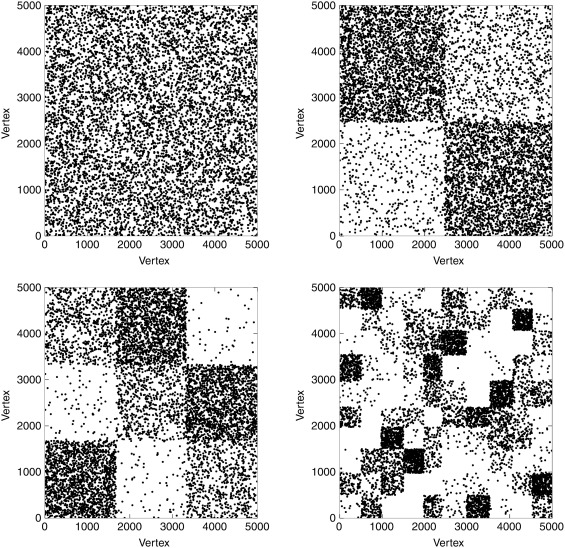
\includegraphics{img/fortunato2016_fig29_randomcommunities.jpg}
\caption{Artificial community structure in a random graph. Each of the
four graphs represent the adjacency matrix of the same 5000-node random
graph, in which every pair of nodes has equal probility of sharing a
link. The top right matrix shows the nodes in arbitrary order, and the
impression is one of random white noise. The others are simply
rearrangements of the nodes for the same random graph. A community
structure can be seen from what is actually random fluctuations in the
network construction process. Figure from
\autocite{fortunato_community_2016}.}\label{fig:randomcommunities}
\end{figure}

This raises the question: how can we be confident that the communities
detected by an algorithm reflect actual community structure, and not an
artifact of random noise? This is an open problem in network science,
but several attempts have been made to address it.

One approach is to compare the results to an appropriate null model. The
most popular null model has been the configuration model, which can
generate any configuration of a network given a number of nodes, number
of edges, and degree assignment for every node. One can use an ensemble
of these networks and compare them against empirical results. Any
measure of the graph, for example a centrality measure of a given node,
can be compared with the same measure on a number of generated null
models; a \(p\)-value can then be calculated as the fraction of model
configurations that yield the same value for the measure as the observed
network \autocite{fortunato_community_2016}. (It may be difficult to
operationalize ``same value'' here---requiring an exact match might make
this test too insensitive, but allowing for variation would introduce
more noise.) One could apply this approach to the community structure as
a whole, or to individual communities, or to community membership of
individual nodes, measuring these phenomena against their presence in an
ensemble of generated graphs.

Another approach is to consider the robustness of a given network to
perturbations in the network structure. From a conceptual standpoint,
this approach differs from the above one in that it does not consider
the network structure as having been generated from a stochastic
process, and attempt to model that process. Rather, it takes the
structure as given and observes the effects of random noise introduced
into this structure on the communities that are detected. This approach
has the advantages that it is applicable to any method, and it is not
restricted to a particular null model
\autocites{rosvall_mapping_2010}{mirshahvalad_significant_2012}.\footnote{In
  practice, however, a particular null model is often implied in a
  perturbation strategy, as can be seen in the discussed examples.}

Several strategies for perturbing networks have been proposed. Gfeller
et al. \autocite{gfeller_finding_2005} employ a strategy on weighted
graphs in which edge weights are increased or decreased by a relative
amount \(0 < \delta < 1\). After choosing \(\delta\), multiple
realizations of the graph are clustered using any method, and the
\emph{in-cluster} probability of each pair of adjacent vertices
\(p_{ij}\) is calculated as the fraction of realizations in which they
were clustered together. Edges with \(p_{ij} < \theta\) are considered
to be \emph{external} edges. This approach has as a weakness the need to
choose values for \(\delta\) and \(\theta\). The authors also provide a
way to measure the overall stability of the partition using these
in-cluster probabilities; this measure needs to be compared against a
null model.

Karrer et al. \autocite{karrer_robustness_2008} use a strategy for
unweighted graphs of network rewiring. Each edge is considered and
either left alone or, with probability \(\alpha\), it is removed and
replaced with another edge between a pair of vertices \((i, j)\) chosen
at random with probability \(p_{ij} = k_i k_j / 2m\) (\(k_i\) and
\(k_j\) are the degrees of \(i\) and \(j\); \(m\) is the number of edges
in the graph). This probability is the same one used in the null model
of modularity. The authors generated multiple graphs for different
values of \(\alpha\), and compared their clusterings to each other using
the variation of information \(V\). They then plotted \(V\) against
\(\alpha\) to see how different levels of perturbation would affect the
stability of the network structure. They compared the function
\(V(\alpha)\) against a null model---again, the null model of
modularity.

Rosvall and Bergstrom use a parametric bootstrap resampling method to
measure significance of communities. To resample the graph, each edge is
assigned a weight from a Poisson distribution with mean equal to the
original edge weight. The authors then cluster both the original and
resampled networks (any clustering method can be used; the authors used
Infomap). Each cluster of the original graph is considered, and of these
nodes the largest subset clustered in the same group in at least 95\% of
the resampled networks is deemed a significant cluster. By applying this
technique on citation graphs at different time points, the authors track
the change in the community structure over time (see subsection
``\protect\hyperlink{networks-of-scholarship}{Networks of scholarship}''
in section ``\protect\hyperlink{applications}{Applications of community
detection}'')

Mirshahvalad et al. \autocite{mirshahvalad_significant_2012} propose a
\emph{constructive} perturbation approach suitable for sparse networks.
These networks have a danger that communities can be ``shattered'' into
small modules if there are missing links due to noise in the data.
\emph{Link prediction} is employed to add links to the network,
strengthening the communities. The link prediction strategy used is
triangle completion, in which a fraction of open triangles are completed
by adding a link. This is a relatively simple strategy, and more
sophisticated methods can be used, but the authors show that it performs
well on benchmark graphs that have been shattered. This method can be
used as a bootstrap resampling technique, and significance can be
measured based on the resampled distribution. A weakness of this method
is that the number of links to be added needs to be chosen, but the
benchmark experiments suggest that results are robust to this choice.

In summary, measuring our confidence in community detection techniques
seems to be a hard problem. Network data are highly interrelated, so
typical independence assumptions that underlie many statistical methods
do not apply. One important issue is the lack of a realistic null model.
Typical null models assume that any node can be connected to any other
with equal probability, but this assumption does not intuitively hold
for large networks. More appropriate would be to have a ``horizon'' of
nodes that each node is more likely to interact with, but such horizons
have yet to be defined \autocite{fortunato_community_2010}. The lack of
appropriate null models is a problem for generative models that rely on
them explicitly, but they tend to underlie assumptions behind link
perturbation and resampling strategies as well. More work remains to be
done to arrive at standard ways of measuring our confidence in the
results of community detection.

\subsection{Algorithmic inaccuracy}\label{algorithmic-inaccuracy}

Our confidence in the performance of a given algorithm due to, for
instance, using different random seeds is a distinct issue. The
statistical significance of community detection is a question of
confidence in the \emph{theory} behind our method. Variation in the
results due to the fact that we are necessarily using approximating
algorithms (due to the complexity of the problem), on the other hand,
affects our confidence in the \emph{implementation} of our method. In
the case of Infomap, during each pass of the core algorithm, the nodes
are considered one at a time in random order, and merged with one of its
neighbors in order to give maximum improvement to the objective function
(the map equation). In principle, there should be one global minimum for
the map equation, corresponding to the one optimal community structure.
In practice, it does seem like the order that the nodes are considered
does make a difference in the final value of the map equation---i.e.,
how well Infomap is able to approximate this global optimum. For
example, in a recent experiment in which I performed 106 runs of Infomap
on the JSTOR article citation network, I found an approximately normal
distribution of final values between 11.334 and 11.364 (mean 11.348,
standard dev 0.00577). These numbers are of course difficult to
interpret, but they do show that there is at least some variation.

The Infomap algorithm is based on the Louvain method for modularity
maximization. In the paper introducing the Louvain method, Blondel el
al. report on this issue. While they see the same type of variation in
relation to the random order, they claim the effect is small, and they
are more concerned with the effect the order has on computation time.
They leave further understanding of the issue to future study
\autocite{blondel_fast_2008}.

In light of this, it would not be a bad idea for someone using any
approximating method to perform multiple runs if she is interested in
finding the best solution possible. More work is needed to understand
specifically the effect of the random seed on the performance of
Infomap.

\clearpage
\hypertarget{pyinfomap}{\section{Infomap implementation in
Python}\label{pyinfomap}}

\protect\hyperlink{pyinfomap}{}

The code I am submitting is my work on a Python implementation of
Infomap: \url{https://github.com/h1-the-swan/pyinfomap}

As far as I know, there does not yet exist a pure Python implementation
of Infomap, the algorithm to detect communities in network data by
minimizing the map equation. The Infomap software, available at
\url{http://www.mapequation.org/code.html}, is written in C++, although
it has extensions in other languages including Python. A Python
repository was created by Daniel Halperin in 2013.\footnote{\url{https://github.com/uwescience/pyinfomap}}
This code, deemed version 1 by Dr.~Halperin, is capable of calculating
the map equation for a given network and a given two-level clustering of
its nodes.\footnote{By ``two-level clustering'', I mean a
  non-hierarchical, non-overlapping partitioning of each node into
  exactly one of any number of clusters.} My code is a fork of this
repository: I coded the algorithm starting with this base code that can
calculate the function to optimize.

The map equation is (see section
\protect\hyperlink{the-dynamical-perspective}{``The dynamical
perspective''} for background):
\[L(\mathsf{M}) = q_{\curvearrowright} H(\mathcal{Q}) + \sum_{i=1}^{m}{p_{\circlearrowright}^{i} H(\mathcal{P}^i)}\]
where \(\mathsf{M}\) is the module partitioning; the left term is the
average length of codewords (entropy) in the index codebook weighted by
the rate of use of the index codebook \(q_{\curvearrowright}\); and the
right term is the average length of codewords in module codebook \(i\)
weighted by the rate of use of this module \(p_{\circlearrowright}\).
Using \(q_{\curvearrowright} = \sum_{i=1}^{m}{q_{i\curvearrowright}}\);
\(p_{\circlearrowright}^{i} = \sum_{\alpha \in i}{p_{\alpha}} + q_{i\curvearrowright}\)
where \(\alpha \in i\) means every node in module \(i\) (the
\(q_{i\curvearrowright}\) is added as the probability that the random
walker exits the module and the exit codeword is used); and the
definition of entropy\footnote{For a random variable \(X\) that can have
  \(n\) states with probability \(p_i\), the entropy is
  \(H(X) = -\sum_{i=1}^{n}{p_i\log{p_i}}\).}, the map equation can be
expanded to: \[
\begin{aligned}
L(\mathsf{M}) = &\left(\sum_{i=1}^{m}{q_{\curvearrowright}}\right) 
                                        \log \left(\sum_{i=1}^{m}{q_{\curvearrowright}}\right)
                                        - 2 \sum_{i=1}^{m}{q_{\curvearrowright}} \log (q_{\curvearrowright)} \\
                                &- \sum_{\alpha=1}^{n}{p_{\alpha} \log(p_\alpha)}
                                        + \sum_{i=1}^{m}{\left(q_{\curvearrowright} + \sum_{\alpha \in i}{p_{\alpha}}\right) \log \left(q_{\curvearrowright} + \sum_{\alpha \in i}{p_{\alpha}}\right)}
\end{aligned}
\]

The node visit probability \(p_{\alpha}\) is related to the dynamics
being modeled. Dr.~Halperin's code uses PageRank with teleportation
probability \(\tau = 0.15\). This is modeling a random walker on the
network that has a 15\% chance, on every step, of teleporting to a
random node instead of following a link as normal. The code uses the
Python package NetworkX \autocite{hagberg_exploring_2008} to handle
graph storage and operations; this package has its own method for
calculating PageRank for every node. The exit probability
\(q_{i\curvearrowright}\) is then calculated as
\autocite{rosvall_map_2010}:
\[q_{i\curvearrowright} = \tau \frac{n-n_i}{n} \sum_{\alpha \in i}{p_{\alpha}} + (1-\tau) \sum_{\alpha \in i}{\sum_{\beta \notin i}{p_{\alpha}w_{\alpha \beta}}}\]
where \(n_i\) is the number of nodes in module \(i\), and
\(w_{\alpha \beta}\) is the normalized weight of the link from
\(\alpha\) to \(\beta\) (if \(\alpha\) is a dangling node, this weight
is replaced by \(1-n_i/n\)).

Version 1 implements a \texttt{Module} class and a \texttt{Clustering}
class. I build a \texttt{PyInfomap} on top of these in order to be able
to calculate the map equation for different clusterings of an input
graph. What follows is my work implementing an optimization algorithm.

The test example I use is network (a) in Fig.~\ref{fig:mapvsmod} in this
document (in the original work \autocite{rosvall_map_2010} it is fig.
3). A pajek version of this network was included in the forked
repository as \texttt{2009\_figure3ab.net}. We know from the text
\autocite{rosvall_map_2010} that the clustering seen in the figure
should have a value for the map equation \(L = 3.33\), and that this is
the optimal (minimum) value for this network. Thus, my algorithm should
be able to find this clustering.

One approach to find the clustering would be to calculate the map
equation for every possible partition of the network. I implement this
in \texttt{search\_all\_possible\_partitions.py}. However, there are far
too many combinations of partitions for network data, even for the small
16-node network I use to test. As of this writing, this code has not yet
finished after running for 212 hours (almost 9 days), having tried over
\(6.15 \times 10^9\) different partitions.

A more realistic option is to use some sort of search algorithm. I
implement the Louvain method, which was originally developed as a
modularity-optimizing community detection algorithm
\autocite{blondel_fast_2008}, and which is the starting point for the
official version of Infomap \autocite{rosvall_map_2010}. This method
consists of two phases, which are performed repeatedly. It starts with
every node in it's own separate module. In the first phase, each node,
one at a time in random order, is moved to be in the same module as its
neighbor that gives the lowest value of the map equation. This is
repeated until no improvement can be made. In the second phase, a new
network is constructed in which the nodes represent the clusters found
in the previous step, edges are weighted by the number of
between-cluster edges in the original graph, and within cluster edges
become self-loops (i.e., edges from one node in the new network to
itself). The algorithm is then repeated on this new graph, with each
calculation of the map equation done using the original graph. Phase one
and two are repeated until no improvement is seen.
Fig.~\ref{fig:louvain} shows a schematic of this procedure.

\begin{figure}
\centering
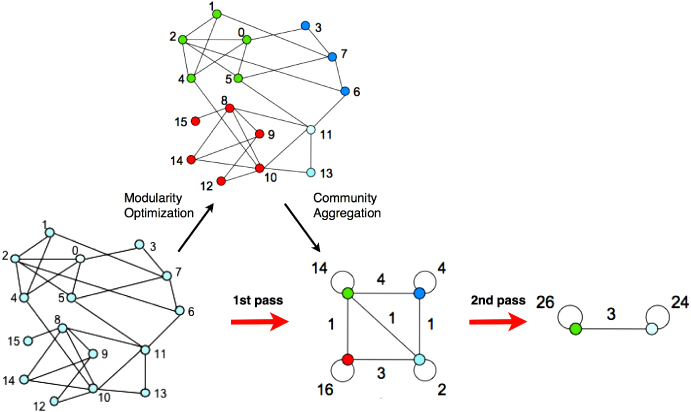
\includegraphics{img/blondel2008_fig1_louvain.jpg}
\caption{Schematic of the Louvain algorithm from
\autocite{blondel_fast_2008}. Each pass consists of a phase in which
local merges of communities are made to optimize the objective function,
and a phase in which a new meta-graph is constructed with the
communities as nodes. The two phases are repeated until no improvement
is found.}\label{fig:louvain}
\end{figure}

The official Infomap algorithm takes additional steps after this point
to broaden the search space and avoid local optima. These include
recursively running the algorithm on the clusters, and freeing
individual nodes to move between modules. My implementation does not yet
include this.

My implementation can find the optimal four-way partition of the test
network. It can also find the optimal partition for network (d) in the
same figure, in which all nodes are grouped into the same module. It
runs in under 1 second on these test networks (after loading the needed
libraries). It is able to run the larger karate club network (34 nodes)
in under 5 seconds.

Next steps would include tests on synthetic benchmarks, and further
analysis of the results of the karate club network, as well as other
standard examples (see section
\protect\hyperlink{evaluation}{``Evaluation of community detection
methods''}).

\clearpage
% END INPUTS

\printbibliography
	
\end{document}
